% arara: lualatex: { shell : yes }
% arara: lualatex: { shell : yes }

\documentclass[a4paper,11pt]{kth-mag}
\DeclareMathSizes{12}{}{}{}

% Math and code packages
\usepackage{amsmath}   % all things math
\usepackage{amssymb}   % additional math symbols
\usepackage{xfrac}     % nice fractions in body of text
\usepackage{siunitx}   % typesets numbers with units
\usepackage{mathtools} % extensions for amsmath
\usepackage[section]{minted}    % advanced code examples

% Tables
\usepackage{booktabs} % professionally looking tables
\usepackage{tabulary} % whole page tables

% Caption and split floats
\usepackage{caption}    % customizable captions
\usepackage{subcaption} % nice subfigures and subtables

% Bibliographies
\usepackage[backend=biber]{biblatex} % modern bibliographies

% PDF Metadata
\usepackage{hyperref} % enables PDF hyperlinks

% Fonts, typography and languages
\usepackage{fontspec}     % all things fonts
\defaultfontfeatures{Ligatures=TeX}
\setmainfont{FiraSans-Book.otf}[
  BoldFont = FiraSans-SemiBold.otf,
  ItalicFont = FiraSans-Italic.otf,
  BoldItalicFont = FiraSans-SemiBoldItalic.otf]
\setsansfont{FiraSans-Regular.otf}[Scale=MatchLowercase]
\setmonofont{FiraMono-Regular.otf}[Scale=MatchLowercase]
\usepackage{unicode-math} % use custom fonts for math
\setmathfont{Asana-Math.otf}
\usepackage{microtype}	  % advanced typesetting
\DisableLigatures{family=tt*}
\usepackage[main=english, swedish]{babel} % language-specific conventions

% Graphics
\usepackage{graphicx} % all things graphics
\usepackage{pgfplots} % complex graphs
\usepackage{pgfplotstable}
\pgfplotsset{
  compat=1.11, % avoid running in backwards compatibility mode
  width=\textwidth,
  tick label style = {font=\ttfamily},
  every axis label = {font=\sffamily},
  legend style = {font=\sffamily},
  label style = {font=\sffamily},
  separate axis lines,
  y axis line style={draw opacity=0},
  x axis line style={gray},
  axis x line*=bottom,
  axis y line*=left,
  major tick length=0pt,
  grid=both,
  y grid style={dashed},
  legend pos=north west,
}
\definecolor{set11}{RGB}{228,  26,  28}
\definecolor{set12}{RGB}{ 55, 126, 184}
\definecolor{set13}{RGB}{ 77, 175,  74}
\definecolor{set14}{RGB}{152,  78, 163}
\definecolor{set15}{RGB}{255, 127,   0}
\definecolor{set16}{RGB}{255, 255,  51}
\definecolor{set17}{RGB}{166,  86,  40}
\definecolor{set18}{RGB}{247, 129, 191}
\definecolor{set19}{RGB}{153, 153, 153}

\definecolor{set11_light}{RGB}{251, 180, 174}
\definecolor{set12_light}{RGB}{179, 205, 227}
\definecolor{set13_light}{RGB}{204, 235, 197}
\definecolor{set14_light}{RGB}{222, 203, 228}
\definecolor{set15_light}{RGB}{254, 217, 166}
\definecolor{set16_light}{RGB}{255, 255, 204}
\definecolor{set17_light}{RGB}{229, 216, 189}
\definecolor{set18_light}{RGB}{253, 218, 236}
\definecolor{set19_light}{RGB}{242, 242, 242}

% \definecolor{set11}{cmyk}{.1 ,.9 ,.8 ,.0 }
% \definecolor{set12}{cmyk}{.8 ,.3 ,.0 ,.0 }
% \definecolor{set13}{cmyk}{.7 ,.0 ,.8 ,.0 }
% \definecolor{set14}{cmyk}{.4 ,.65,.0 ,.0 }
% \definecolor{set15}{cmyk}{.0 ,.5 ,1.0,.0 }
% \definecolor{set16}{cmyk}{.0 ,.0 ,.8 ,.0 }
% \definecolor{set17}{cmyk}{.35,.6 ,.8 ,.0 }
% \definecolor{set18}{cmyk}{.0 ,.5 ,.0 ,.0 }
% \definecolor{set19}{cmyk}{.0 ,.0 ,.0 ,.4 }
%
% \definecolor{set11_light}{cmyk}{.0 ,.3 ,.2 ,.0 }
% \definecolor{set12_light}{cmyk}{.3 ,.1 ,.0 ,.0 }
% \definecolor{set13_light}{cmyk}{.2 ,.0 ,.2 ,.0 }
% \definecolor{set14_light}{cmyk}{.12 ,.17,.0 ,.0 }
% \definecolor{set15_light}{cmyk}{.0 ,.15 ,.3,.0 }
% \definecolor{set16_light}{cmyk}{.0 ,.0 ,.2 ,.0 }
% \definecolor{set17_light}{cmyk}{.1,.12 ,.2 ,.0 }
% \definecolor{set18_light}{cmyk}{.0 ,.15 ,.0 ,.0 }
% \definecolor{set19_light}{cmyk}{.0 ,.0 ,.0 ,.05 }

\usepackage{modifications}

\linespread{1.2}

\title{GPU Simulation of Rigid Fibers}

\foreigntitle{GPU simulering av stela fibrer}

\author{Eric Wolter}
\date{January 2015}
\blurb{Master's Thesis at School of Engineering Sciences\\Supervisor: Katarina Gustavsson\\Examiner: Michael Hanke}
\trita{TRITA xxx yyyy-nn}

\begin{document}
\frontmatter
\pagestyle{empty}

\maketitle
\selectlanguage{english}
\begin{abstract}
Lorem ipsum dolor sit amet, consectetuer adipiscing elit. Mauris
purus. Fusce tempor. Nulla facilisi. Sed at turpis. Phasellus eu
ipsum. Nam porttitor laoreet nulla. Phasellus massa massa, auctor
rutrum, vehicula ut, porttitor a, massa. Pellentesque fringilla. Duis
nibh risus, venenatis ac, tempor sed, vestibulum at, tellus. Class
aptent taciti sociosqu ad litora torquent per conubia nostra, per
inceptos hymenaeos.
\end{abstract}

\clearpage


\begin{foreignabstract}{swedish}
Lorem ipsum dolor sit amet, consectetuer adipiscing elit. Mauris
purus. Fusce tempor. Nulla facilisi. Sed at turpis. Phasellus eu
ipsum. Nam porttitor laoreet nulla. Phasellus massa massa, auctor
rutrum, vehicula ut, porttitor a, massa. Pellentesque fringilla. Duis
nibh risus, venenatis ac, tempor sed, vestibulum at, tellus. Class
aptent taciti sociosqu ad litora torquent per conubia nostra, per
inceptos hymenaeos.
\end{foreignabstract}

\clearpage

\tableofcontents*

\clearpage

\listoflistings

\mainmatter
\pagestyle{newchap}

\chapter{Introduction}

% \begin{figure}
%   \centering
%   \begin{tikzpicture}
%     \setmathfont{FiraSans-Book.otf}
%     \begin{axis}[
%       title=Overall,
%       xlabel={number of fibers},
%       ylabel={simulation time (sec)},
%       xmin=0,xmax=700,
%       ymin=0,ymax=16,
%       unbounded coords=discard,
%       ]
%     \addplot[set11,mark=*,mark options={fill=white}, very thick] table[x=X,y expr=\thisrow{TOTAL} * 0.125] {benchmarks/katarina_gmres_analytical.csv};
%     \addplot[set12,mark=*,mark options={fill=white}, very thick] table[x=X,y=total]  {benchmarks/cuda_gmres_numerical_2D.csv};
%     \addplot[set13,mark=*,mark options={fill=white}, very thick] table[x=X,y=total]  {benchmarks/cuda_bicgstab_numerical_2D.csv};
%     % \addplot[set14,mark=*,mark options={fill=white}, very thick] table[x=X,y=total]  {benchmarks/cuda_magma_numerical_2D.csv};
%     % \addplot[set15,mark=*,mark options={fill=white}, very thick] table[x=X,y=TOTAL] {benchmarks/openmp_direct_numerical.csv};
%     % \addplot[set16,mark=*,mark options={fill=white}, very thick] table[x=X,y=TOTAL] {benchmarks/openmp_direct_analytical.csv};
%
%     \legend{Fortran (Original\, Linear Scaling), CUDA (GMRES\, Numerical\, 2D), CUDA (BiCGStab\, Numerical\, 2D), CUDA (MAGMA\, Numerical\, 2D), OpenMP (Direct\, Numerical), OpenMP (Direct\, Analytical)}
%     \end{axis}
%     \setmathfont{XITS Math}
%   \end{tikzpicture}
%   \caption{Total time per timestep using the average over 10 timesteps. First timestep is excluded as warmup. Assuming linear scaling for Fortran.}
% \end{figure}
%
% \begin{figure}
%   \centering
%   \begin{tikzpicture}
%     \setmathfont{FiraSans-Book.otf}
%     \pgfplotstableread{benchmarks/cuda_magma_numerical_2D.csv}\loadedtable
%     \begin{axis}[
%       stack plots=y,
%       area style,
%       title=Steps (CUDA Magma),
%       xlabel={number of fibers},
%       ylabel={simulation time (sec)},
%       xmin=0,xmax=700,
%       ymin=0,ymax=3,
%       ]
%     \addplot[color=set11, fill=set11_light, very thick] table[x=X,y=assemble_system] {\loadedtable} \closedcycle;
%     \addplot[color=set12, fill=set12_light, very thick] table[x=X,y=solve_system] {\loadedtable} \closedcycle;
%     % update_fibers is so small it just causes ugly undefined jagginess of the lines
%     % so we just add it to update velocities and rename both to update system
%     \addplot[color=set13, fill=set13_light, very thick] table[x=X,y expr=\thisrow{update_velocities} + \thisrow{update_fibers}] {\loadedtable} \closedcycle;
%     % \addplot[color=set14, fill=set14_light, very thick] table[x=X,y=update_fibers] {\loadedtable} \closedcycle;
%
%     \legend{Assemble System, Solve System (MAGMA), Update System}
%     \end{axis}
%     \setmathfont{XITS Math}
%   \end{tikzpicture}
%   \caption{Average time for each simulation step over 10 timesteps. First timestep is excluded as warmup.}
% \end{figure}
%
% \begin{figure}
%   \centering
%   \begin{tikzpicture}
%     \setmathfont{FiraSans-Book.otf}
%     \pgfplotstableread{benchmarks/katarina_gmres_analytical.csv}\loadedtable
%     \begin{axis}[
%       stack plots=y,
%       area style,
%       title=Steps (Fortran Original),
%       xlabel={number of fibers},
%       ylabel={simulation time (sec)},
%       xmin=0,xmax=700,
%       ymin=0,ymax=110,
%       ]
%     \addplot[color=set11, fill=set11_light, very thick] table[x=X,y=ASSEMBLE_MATRIX] {\loadedtable} \closedcycle;
%     \addplot[color=set12, fill=set12_light, very thick] table[x=X,y=SOLVE_SYSTEM] {\loadedtable} \closedcycle;
%     % update_fibers is so small it just causes ugly undefined jagginess of the lines
%     % so we just add it to update velocities and rename both to update system
%     \addplot[color=set13, fill=set13_light, very thick] table[x=X,y expr=\thisrow{UPDATE_VELOCITIES} + \thisrow{UPDATE_FIBERS}] {\loadedtable} \closedcycle;
%     % \addplot[color=set14, fill=set14_light, very thick] table[x=X,y=update_fibers] {\loadedtable} \closedcycle;
%
%     \legend{Assemble System, Solve System, Update System}
%     \end{axis}
%     \setmathfont{XITS Math}
%   \end{tikzpicture}
%   \caption{Average time for each simulation step over 10 timesteps. First timestep is excluded as warmup. Assuming linear scaling for Fortran.}
% \end{figure}
%
% \begin{figure}
%   \centering
%   \begin{tikzpicture}
%     \setmathfont{FiraSans-Book.otf}
%     \pgfplotstableread{benchmarks/openmp_direct_analytical.csv}\loadedtable
%     \begin{axis}[
%       stack plots=y,
%       area style,
%       title=Steps (OpenMP analytical),
%       xlabel={number of fibers},
%       ylabel={simulation time (sec)},
%       xmin=0,xmax=700,
%       ymin=0,ymax=9,
%       ]
%     \addplot[color=set11, fill=set11_light, very thick] table[x=X,y=ASSEMBLE_SYSTEM] {\loadedtable} \closedcycle;
%     \addplot[color=set12, fill=set12_light, very thick] table[x=X,y=SOLVE_SYSTEM] {\loadedtable} \closedcycle;
%     % update_fibers is so small it just causes ugly undefined jagginess of the lines
%     % so we just add it to update velocities and rename both to update system
%     \addplot[color=set13, fill=set13_light, very thick] table[x=X,y expr=\thisrow{UPDATE_VELOCITIES} + \thisrow{UPDATE_FIBERS}] {\loadedtable} \closedcycle;
%     % \addplot[color=set14, fill=set14_light, very thick] table[x=X,y=update_fibers] {\loadedtable} \closedcycle;
%
%     \legend{Assemble System, Solve System, Update System}
%     \end{axis}
%     \setmathfont{XITS Math}
%   \end{tikzpicture}
%   \caption{Average time for each simulation step over 10 timesteps. First timestep is excluded as warmup. Assuming linear scaling for Fortran.}
% \end{figure}
%
% \begin{figure}
%   \centering
%   \begin{tikzpicture}
%     \setmathfont{FiraSans-Book.otf}
%     \begin{axis}[
%       title=Solve System Comparison,
%       xlabel={number of fibers},
%       ylabel={simulation time (sec)},
%       xmin=0,xmax=700,
%       ymin=0,ymax=6,
%       ]
%     \addplot[color=set11,mark=*,mark options={fill=white}, very thick] table[x=X,y expr=\thisrow{SOLVE_SYSTEM} * 0.125] {benchmarks/katarina_gmres_analytical.csv};
%     \addplot[color=set12,mark=*,mark options={fill=white}, very thick] table[x=X,y=solve_system]  {benchmarks/cuda_gmres_numerical_2D.csv};
%     \addplot[color=set13,mark=*,mark options={fill=white}, very thick] table[x=X,y=solve_system]  {benchmarks/cuda_bicgstab_numerical_2D.csv};
%     \addplot[color=set14,mark=*,mark options={fill=white}, very thick] table[x=X,y=solve_system]  {benchmarks/cuda_magma_numerical_2D.csv};
%     \addplot[color=set15,mark=*,mark options={fill=white}, very thick] table[x=X,y=SOLVE_SYSTEM] {benchmarks/openmp_direct_numerical.csv};
%
%     \legend{Solve System (Fortran\, Original\, GMRES), Solve System (CUDA\, GMRES), Solve System (CUDA\, BiCGStab), Solve System (CUDA\, MAGMA), Solve System (OpenMP\, OpenBLAS)}
%     \end{axis}
%     \setmathfont{XITS Math}
%   \end{tikzpicture}
%   \caption{Average time for solve system step. Averaged over 10 timesteps (1st excluded). Assuming linear scaling for Fortran.}
% \end{figure}
%
% \begin{figure}
%   \centering
%   \begin{tikzpicture}
%     \setmathfont{FiraSans-Book.otf}
%     \begin{axis}[
%       title=Assemble System Comparison,
%       xlabel={number of fibers},
%       ylabel={simulation time (sec)},
%       xmin=0,xmax=700,
%       ymin=0,ymax=8
%       ]
%     \addplot[color=set11,mark=*,mark options={fill=white}, very thick] table[x=X,y expr=(\thisrow{ASSEMBLE_MATRIX} + \thisrow{ASSEMBLE_RHS}) * 0.125] {benchmarks/katarina_gmres_analytical.csv};
%     \addplot[color=set12,mark=*,mark options={fill=white}, very thick] table[x=X,y=assemble_system] {benchmarks/cuda_magma_numerical_2D.csv};
%     \addplot[color=set13,mark=*,mark options={fill=white}, very thick] table[x=X,y=assemble_system] {benchmarks/cuda_bicgstab_analytical_2D.csv};
%     \addplot[color=set14,mark=*,mark options={fill=white}, very thick] table[x=X,y=ASSEMBLE_SYSTEM] {benchmarks/openmp_direct_numerical.csv};
%     \addplot[color=set15,mark=*,mark options={fill=white}, very thick] table[x=X,y=ASSEMBLE_SYSTEM] {benchmarks/openmp_direct_analytical.csv};
%
%     \legend{Assemble System (Fortran\, Analytical), Assemble System (CUDA\, Numerical), Assemble System (CUDA\, Analytical), Assemble System (OpenMP\, Numerical), Assemble System (OpenMP\, Analytical)}
%     \end{axis}
%     \setmathfont{XITS Math}
%   \end{tikzpicture}
%   \caption{Average time for assemble system step. Fortran and CUDA are averaged over 10 timesteps (1st excluded). Fortran New is only 1st timestep. Assuming linear scaling for Fortran.}
% \end{figure}
%
%
% \begin{figure}
%   \centering
%   \begin{tikzpicture}
%     \setmathfont{FiraSans-Book.otf}
%     \pgfplotstableread{benchmarks/assemble_system_grid.csv}\loadedtable
%     \begin{axis}[
%       title=CUDA Grid Dimension,
%       xlabel={number of fibers},
%       ylabel={simulation time (sec)},
%       ymin=0,ymax=0.8,
%       xmin=0,xmax=700,
%       unbounded coords=discard,
%       ]
%     \addplot[set11,mark=*,mark options={fill=white}, very thick] table[x=X,y=1D] {\loadedtable};
%     \addplot[set12,mark=*,mark options={fill=white}, very thick] table[x=X,y=2D] {\loadedtable};
%     \addplot[set13,mark=*,mark options={fill=white}, very thick] table[x=X,y=3D] {\loadedtable};
%     \addplot[set14,mark=*,mark options={fill=white}, very thick] table[x=X,y=3D2] {\loadedtable};
%
%     \legend{1D, 2D, 3D, 3D2}
%     \end{axis}
%     \setmathfont{XITS Math}
%   \end{tikzpicture}
%   \caption{Total time per timestep using the average over 10 timesteps. First timestep is excluded as warmup.}
% \end{figure}

\chapter{Theoretical Foundation}
\label{cha:theoretical_foundation}
The introduction discussed the various applications of the rigid fiber simulations. It stressed the importance of being able to simulate as many fibers as possible to generate the interesting patterns found in real world experiments.

In this chapter I will present the required theoretical foundation of the physics behind the simulation. This is required to be able to understand the numerical method used throughout the rest of the thesis.

I will begin by introducing the Stokes flow and its foundatmental solutions as they apply to slender bodies. Afterwards I will focus on the implications this has and how the flow properties can be calulated for the special case of rigid fibers.

\section{Stokes flow and Stokeslet}
The fluids involved in the rigid fiber simulation are characterized by three properties which allow the general Naviar-Stokes Equations to be immensly simplified.
\begin{enumerate}
  \item{\textit{Newtonian fluid} — The viscosity $\mu$ of the fluid does not depend on the stress.}
  \item{\textit{Incompressible flow} — The density of the fluid does not change.}
  \item{\textit{Low Reynolds number $Re \ll 1$} — The fluid velocities are very slow and/or the viscosity is very large.}
\end{enumerate}

Given these constraints and special case of very low Reynolds numbers the general Naviar-Stokes Equations can be linearized to the Stokes Equations

\begin{equation}
\label{eq:stokes_equations}
\begin{aligned}
    grad(p) - \mu \Delta \mathbf{u} &= \mathbf{f} \quad &\text{in} \quad \Omega \text{,}\\
    div(\mathbf{u}) &= 0 \quad &\text{in} \quad \Omega \text{,}
\end{aligned}
\end{equation}

where $\mathbf{u}(\mathbf{x})$ denotes the velocity field, $p(\mathbf{x})$ the pressure field and $\mathbf{f}(\mathbf{x})$ the force acting on the fluid at the location $\mathbf{x} = (x,y,z) \in \mathbb{R}^3$.
The constant $\mu$ is the viscosity of the fluid.

The Stokes Equations are linear in both the velocity and pressure, which allow them to be solved using a number of different methods for linear differential equations. Additionally the equations are time indepdent and time depedence is only reintroduced by boundary conditions. Thus given the boundary conditions the structure of the flow is can be calculated.

By taking advantage of the linearity of the Stokes equations, which implies the existence of a Green's function, and introducing boundary conditions so called fundamental solutions can be found. First no-slip conditions on the surface of the slender bodies are defined as
\begin{equation}
  \label{eq:boundary_condition_surface}
  \mathbf{u} = \mathbf{u}_\Gamma  \quad \text{on} \quad  \Gamma \text{,}
\end{equation}
where $\Gamma$ denotes the union of all body surfaces and $\mathbf{u}_\Gamma$ the corresponding surface velocity, thus forcing the fluid to have zero velocity relative to the surface boundary.

Furthermore the velocity field should be equal to a background velocity $\mathbf{U}_0(\mathbf{x})$ at infinity

\begin{equation}
  \label{eq:boundary_condition_background}
  \mathbf{u} \rightarrow \mathbf{U}_0 \quad \text{as} \quad ||\mathbf{u}|| \rightarrow \infty \text{.}
\end{equation}
Next the force term in \eqref{eq:stokes_equations} is replaced by a point force acting at the origin $\mathbf{x}_0$
\begin{equation}
  \label{eq:stokes_equations_point}
  \begin{aligned}
    grad(p) - \mu \Delta \mathbf{u} &= \mathbf{F} \cdot \delta(\mathbf{x} - \mathbf{x}_0) \text{,}\\
    div(\mathbf{u}) &= 0 \text{,}
  \end{aligned}
\end{equation}
where $\delta(\mathbf{x} - \mathbf{x}_0)$ is Dirac delta function. Solving these equations for the velocity field $\mathbf{u}(\mathbf{x})$ yields the fundamental solution
\begin{equation}
  \label{eq:stokeslet}
  \begin{aligned}
    \mathbf{u}(\mathbf{x}) &= \mathbf{S}(\mathbf{x}-\mathbf{x}_0) \text{,}\\
    \mathbf{S}(\mathbf{r}) &= \frac{1}{8\pi\mu} \left(\frac{\mathbf{I}}{|r|} + \frac{rr}{|r|^3}\right) \text{,}
  \end{aligned}
\end{equation}
where $\mathbf{S}$ denotes the Stokeslet tensor and $\mathbf{I}$ the identy tensor. Additionally we will later need to higher order fundamental solutions which can be obtained by simply differentiating the Stokeslet, e.g. the so called doublet is defined as
\begin{equation}
  \label{eq:doublet}
  \mathbf{D}(\mathbf{r}) = \frac{1}{2} \Delta\mathbf{S}(\mathbf{r}) = \frac{1}{8\pi\mu} \left(\frac{\mathbf{I}}{|r|^3} - \frac{3rr}{|r|^5}\right) \text{.}
\end{equation}

\section{Slender bodies}
\section{Rigid fibers}
\subsection{Nondimensionalization}
\subsection{Slender body equations}
\subsection{Forces}
\subsection{Velocities}

\chapter{Serial Implementation}
\label{cha:serial_implementation}

In the last chapter I presented the theoretical foundation of the physics and math involved in simulating rigid fibers. It showed how based on the Stokes Equation a framework can be developed to efficiently model rigid fibers.

Using this background I will now introduce the approach used for the numeric simulation. This is crucial to be able to validate the framework against real world experiments.

I will begin by presenting the employed time stepping approach. This is followed by a discussion about the different ways the integrals can be solved for the various quadrature points. The final section will illustrate the structure of the final obtained linear system and the shortly introduce the employed solvers.

\section{Time stepping}
\section{Quadrature}
\subsection{Numeric Integration}
\subsection{Analytic Integration}
\section{Linear system}

\chapter{Parallel Implementation}
In the previous chapter the implementation of the numerical simulation was discussed. It discussed various implementation details which have to be considered to arrive at the most efficent and performant implementation.

Based on the previous existing serial Fortran implementation this chapter will look at the algorithm in more detail and show how it was adapted to take advantage of multi-core architectures. The main focus of this thesis is the implementation
on modern nVidia GPUs using CUDA. In addition to the main work of reimplementing the algorithm for CUDA and to have a better understanding of the achievable performance improvements the finished GPU code was also ported to multiple CPUs using the OpenMP framework.

I will begin with a short introducing to general purpose computing on the GPU and explain briefly how CUDA works. I then move on to illustrate the practical implementation of the CUDA code. This is followed by a brief explanation of OpenMP and how the code was parallized on the CPU. The chapter ends with the discussion of several potential optimization approaches to further improve the performance of the simulation.

\section{GPU Programming}
In the beginning of Graphics Processing Units were highly specialized pieces of hardware developed to exclusively improve the performance of real-time 3D graphics. However in recent years GPUs have started to be able to run arbitrary code instead of being limited to graphics related computations. GPUs can achieve impressive performance increases across a wide range of different applications. The deciding factor is how well the problem can be parallized to take advantage of the massively parallel architectures of GPUs. This has lead to potentially large performance advantages of GPUs over CPUs as illustrated in figure~\ref{fig:gpu_performance}.

\begin{figure}
  \centering
  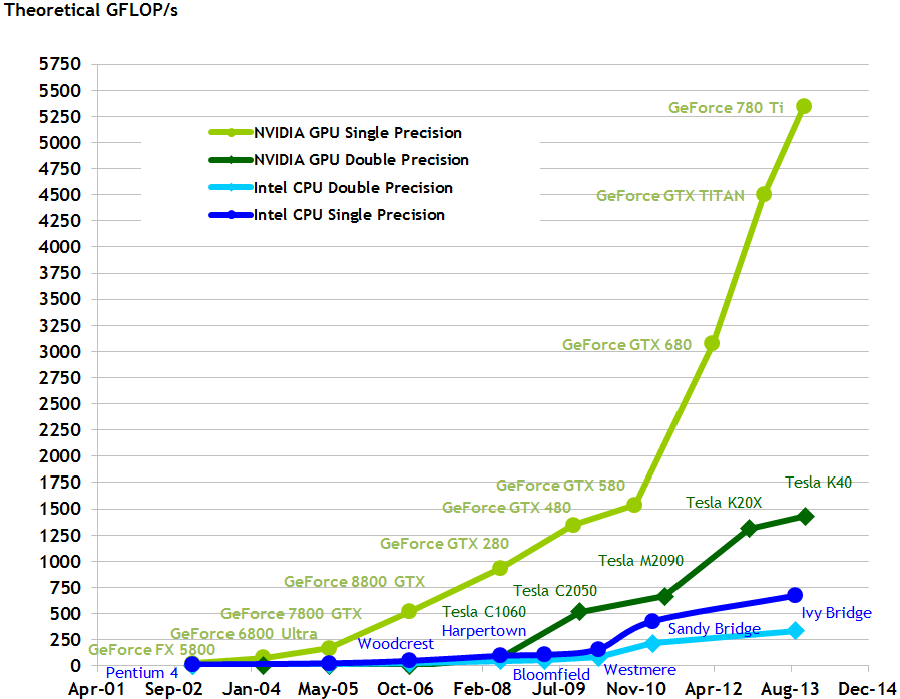
\includegraphics[width=\textwidth]{img/gpu_performance.pdf}
  \caption{Increase in floating-point operations per second for CPUs versus GPUs over time.}
  \label{fig:gpu_performance}
\end{figure}

In contrast to traditional CPUs which have four, eight and sometimes very fast compute cores, GPU can have many hundreds of independt compute cores. Each core can simulatenously perform calculations and thus provides the opportunity to yield big performance improvements for high-throughput type computations. This fact also introduced general purpose computing on GPUs to the world of supercomputers with more and more of them either supplimenting GPUs or even exclusively relying on GPUs for their computations.

In order to take advantage of these new massively parallel architectures new Application Programming Interfaces had to be developed. The two proposed APIs are OpenCL and CUDA. OpenCL is an open and cross platform standard maintained by the Khronos Group. The same group also responsible for its graphics focused counterpart OpenGL. OpenCL is not exclusive to GPUs, but instead tries to be a general abstract layer for different parallel architectures. This allows OpenCL code to be run not only on GPUs but also on CPUs and other new hardware like Intels Xeon Phi. CUDA on the other hand is developed by Nvidia exclusively for their line of GPUs.

Choosing between OpenCL and CUDA is the first decision to be made when starting to implement a new project on GPUs. The main advantage of OpenCL is the ability to be able to run many different devices. Both Intel and AMD provide the API for their processors and both AMD and Nvidia have drivers available for their GPUs. However this advantage can actually also be a disadvantage as the achievable performance might suffer from the abstraction across all these different kinds of devices being not optimized for a particulars device specific architecture. CUDA on the other hand is in theory highly optimized to achieve the best possible performance on Nvidia's GPUs. In practice the difference might be able to be mitigated by spending the extra time to fine tune the OpenCL implementation to the hardware specific needs. Another disadvantage of OpenCL is the potentially outdated and inconsistent driver support for the various devices. This is especially true for Nvidia which seem to have stopped updating OpenCL, still only supporting OpenCL 1.1 which was released back in 2010. Their main focus is on pushing CUDA and updating it to support all the feature in their new GPUs.

For this thesis I chose to go with Nvidia's CUDA framework mainly because of the available hardware both at the workstation computers as well as at the local computing cluster. Additionally this project does not need the cross-platform capability as the main focus is on pure performance in a highly speciliazed setup and simulation scenario. The application will not be widely distributed and only used for internal purposes.

\section{CUDA}
The Compute Unified Device Architecture (CUDA) was introduced by Nvidia in 2006 as a general purpose parallel computing platform. It leverages the highly parallel architecture of modern Nvidia GPUs to solve many different computational problems, which can lead to potentially large performance improvements compared to traditional CPUs.

The CUDA platform allows developers to use a varity of different options to program the GPU. The easiest way is to simply link to any CUDA-accerlated library and simply using the libraries interfaces from any software environment. For more advanced uses extensions to various programming languages exist like C/C++, Fortran and even managed languages like Java and Python and many more. This allows for easy and fast integrating into whatever software environment the developer is comfortable with. figure~\ref{fig:cuda_overview} illustrated the different components of the overall CUDA platform.

\begin{figure}
  \centering
  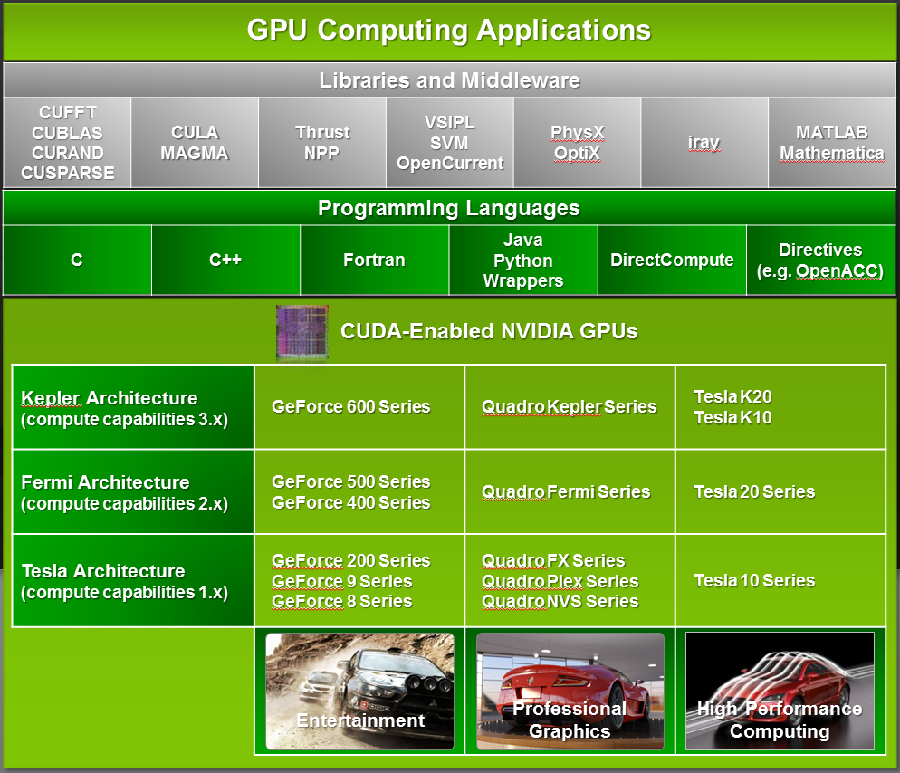
\includegraphics[width=\textwidth]{img/cuda_overview.pdf}
  \caption{Overview of the CUDA platform.}
  \label{fig:cuda_overview}
\end{figure}

The basic building blocks of the CUDA Programming Model from a development perspective are so called kernels. CUDA kernels are the equivalent of normal C functions, however instead of being executed just once. Kernels are executed in parallel by $N$ different threads. These CUDA threads are distributed and run across the available compute cores of the GPU. To illustrate how a very basic kernel call looks see the code sample in Figure \ref{lst:code_vector_addition} for a very simple vector addition.

\paragraph{CUDA Kernels}

\begin{listing}
  \centering
  \begin{minted}[mathescape,
    linenos,
    numbersep=5pt,
    frame=lines,
    framesep=2mm]{c}
// Kernel definition
__global__ void VecAdd(float *A, float *B, float *C)
{
  int i = threadIdx.x;
  C[i] = A[i] + B[i];
}

int main()
{
  ...
  // Kernel invocation with N threads
  VecAdd<<<1,N>>>(A,B,C);
  ...
}
  \end{minted}
  \caption{Pseudocode for CUDA vector addition}
  \label{lst:code_vector_addition}
\end{listing}

It is important to remember that each kernel invocation is executed independently and no ordering is guaraentedd. It is therefore essential to make sure to avoid any race conditions or shared memory access. There are ways to allow for shared memory access which will be briefly touched upon later in the practical implementation of the simulation.

\paragraph{Thread hierarchy}

In order to efficiently distribute the different threads across the compute cores of the GPU, CUDA defines a thread hierachy. As discussed previously a GPU consists of many indepent compute cores. On Nvidia GPUs theses cores are referred to as Streaming Multiprocessors (SMs). During execution of the application each SM is tasked with running a distinct set of threads. In CUDA these sets of threads are called thread blocks. Each thread block is then distributed to all the available SMs, which allows for automatic scalability depending on the number of SMs available on the specfic GPU device as illustrated in figure~\ref{fig:automatic_scaling}.

\begin{figure}
  \centering
  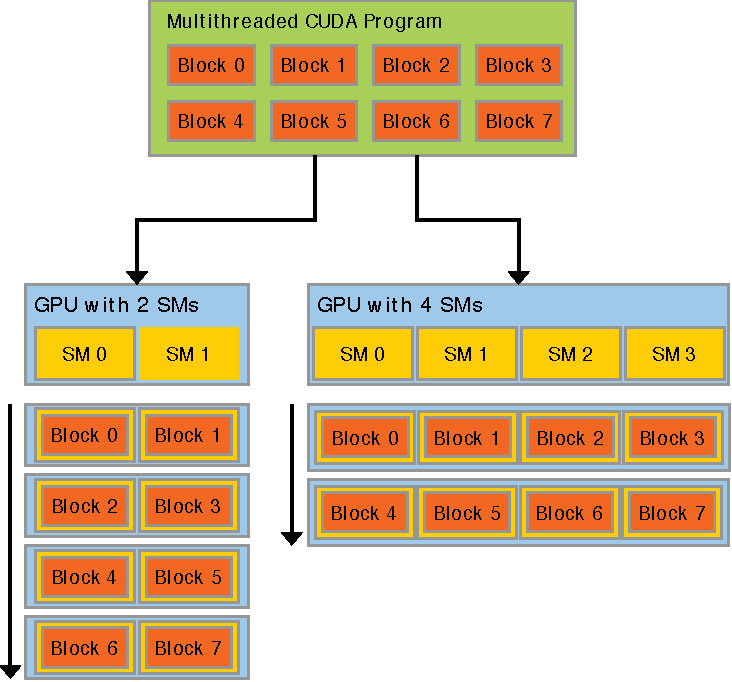
\includegraphics[width=\textwidth]{img/automatic_scaling.pdf}
  \caption{Automatic scaling of blocks across an arbritrary number of Streaming Multiprocessors.}
  \label{fig:automatic_scaling}
\end{figure}

Thus the developer only has to divide the workload into appropiately sized blocks of threads and invoce the kernel. How to choose the optimal size of a block to maximize the performance is not an easy question to answer and is highly dependent on the particular implementation and type of work being done. In practice the size is often chosen by running benchmarks with various different size to determine the sweet spot.

In order to make programming and modeling of real world problems easier CUDA blocks can be addressed using either a one-dimensional, two-dimensional, or three-dimensional thread index. For example in the case of a matrix calculation it is more natural to think about parallezing each element given by the row and column index instead of a single one-dimensional index. This is illustrated in the code simple in listing~\ref{lst:code_matrix_addition}

\begin{listing}
  \centering
  \begin{minted}[mathescape,
    linenos,
    numbersep=5pt,
    fontsize=\footnotesize,
    frame=lines,
    framesep=2mm]{c}
// Kernel definition
__global__ void MatAdd(float A[N][N], float B[N][N], float C[N][N])
{
  int i = threadIdx.x;
  int j = threadIdx.y;
  C[i][j] = A[i][j] + B[i][j];
}

int main()
{
  ...
  // Kernel invocation with one block of N * N * 1 threads
  int numBlocks = 1;
  dim3 threadsPerBlock(N, N);
  MatAdd<<<numBlocks, threadsPerBlock>>>(A,B,C);
  ...
}
  \end{minted}
  \caption{Pseudocode for CUDA matrix addition, illustrating 2D thread blocks}
  \label{lst:code_matrix_addition}
\end{listing}

Finally because the resources of each Streaming Multiprocessor are limited there exists a upper bound of how many threads a block can contain. Currently is maximum number of threads is $1024$. This means that the maximum size of matrices possible to be added in the code sample in listing~\ref{lst:code_matrix_addition} is $32\times32$. To solve this problem CUDA introduces another layer above blocks called a grid. Grid organize thread blocks again into either one, two, or three dimensions. The number of thread blocks in a grid is unlimited and thus solely dependent on the size of the workload. Listing~\ref{fig:grid_blocks} illustrates an example configuration of a 2D grid with 2D blocks.

\begin{figure}
  \centering
  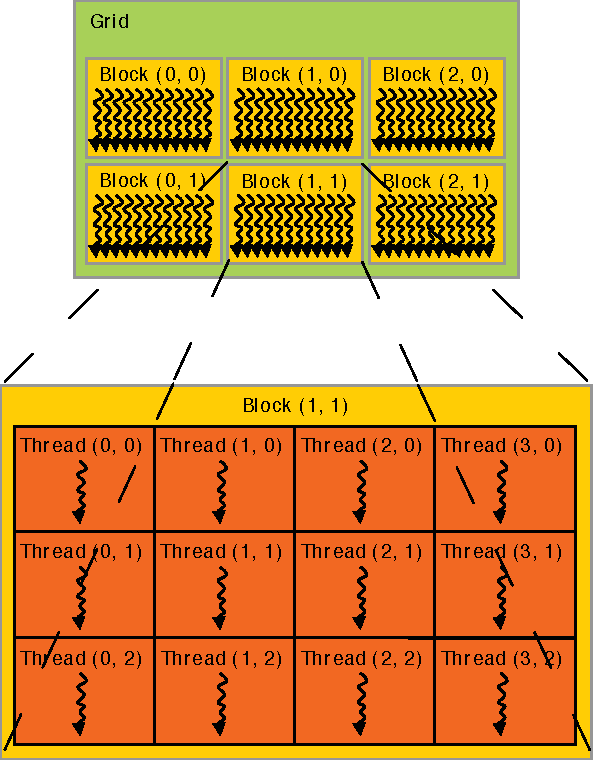
\includegraphics[width=0.6\textwidth]{img/grid_blocks.pdf}
  \caption{Overview of the CUDA platform.}
  \label{fig:grid_blocks}
\end{figure}

\paragraph{Memory hierarchy}

In addition to the Thread hiearchy...

\section{Implementation}
The rigid fiber simulation developed as part of this thesis is only loosely based on the original serial Fortran implementation. This was done to to ensure a clean starting point and avoid difficulties in adapting the existing code for parallel execution as it was never intended to be run across multiple cores. This also provided the opportunity to learn from the shortcomings of the old code to not only parallize it but also improve the efficiency in general.

The development was done exclusively on a Linux workstation running Ubuntu as this will also be the exact same runtime enviroment used in the later experiemntal usage of the resulting application. The build system for compiling and linking the final application was CMake, as it is a widely used open-source and cross-platform build system, allowing for easy integration of the various required libraries in a well documented and straightforward manner.

Under the hood the build system used Nvidia's CUDA platform tools to compile the code using \emph{nvcc}, the Nvidia's LLVM-based CUDA compiler. In addition to the CUDA libraries the application also requires support libraries for the different linear solvers. The two main libraries are \emph{MAGMA} for the direct solver and \emph{ViennaCL} for the iterative solvers. Both will be introduced briefly now.

\paragraph{MAGMA / CuBLAS / OpenBLAS}
The MAGMA project provides the implementation for the direct solver used during this thesis. This dense linear algebra library provides features similar to standard LAPACK functions but for multicore architectures. It also provides features to support hybrid algorithms across multiple different archictures, however these features where not explored in this thesis. Instead the focus was on a high performant single GPU implementation of a direct linear system solver.

MAGMA provides the interfaces for various high-level languages, however the underlying math functions utilize the platform specific implementations of the BLAS levels. For CUDA this is provided directly by Nvidia in the form of the CuBLAS libraries. Additionally MAGMA tries to be as fast as possible which sometimes means integrating CPU based algorithm where it makes sense. Thus a CPU based BLAS implementation is also needed. For this I chose the OpenBLAS library which is the most up to date and high performant library available outside the very expensive Intel MKL library. OpenBLAS takes full advantage of multicore systems using pthreads and is also used for the comparison of Fortran CPU implementation against the CUDA GPU implementation

\paragraph{ViennaCL}
ViennaCL is an open-source linear algebra library developed at the Universiy of Vienna. The library provides an abstraction layer across many different parallization methods in order to provide consistent and easy to use support for BLAS level 1-3 and iterative solvers. This unique feature allows the developer to easily switch between different backends for parallelization. Currentely the library support OpenMP, OpenCL and most importantanly for this thesis CUDA.

While mostly focussed on sparse matrices for the implemented iterative solvers, ViennaCL also support solving dense matrices using a variety of different iterative solvers. As the rigid fiber simulation exclusive relies on dense matrices this makes it an ideal candidate for benchmarking. For this thesis both the BiCGStab as well as the GMRES iterative solvers where used and tested.

In order to faciliate easier usage of application both during development and later real-world usage a Python wrapper script is also available. The script completely automates the building process and dynamically customizes the application code to support three different modes of operation. The first is a simple \emph{run} mode which simply takes the supplied parameters and executes the simulation. The second mode is \emph{validate}, it allows for a fully automated way to test and validate different algorithm variantions against a known correct simulation run. This includes automatically computing the error as well as the error location in the matrix allowing for easier debugging of changes. The last mode is \emph{benchmark} which run the supplied parameters through a series of iterations collecting and aggregating timings for each simulation step as well as the total time.

Unified interface for OpenMP and CUDA -> OpenMP only introduced later?!? -> Is that really important any way?

\subsection{Kernels}
The overall parallel algorithm is very similar to the serial version, however each simulation step is seperated into different kernels. Each kernel is invocate in a serial manner, this means CUDA guarantess that all data modified in a kernel is available before the next kernel is executed. These kernels are than distributed across the GPU. All calculations are done using single precision floating point numbers, as Nvidia limits high performance double precision computation to their server class GPUs. The CUDA pseudocode for algorithm is illustrated in listing~\ref{lst:pseudo_parallel_algorithm}.

\begin{listing}
  \centering
  \begin{minted}[mathescape,
    linenos,
    numbersep=5pt,
    fontsize=\footnotesize,
    frame=lines,
    framesep=2mm]{c}
int main()
{
  // Parsing algorithm parameters and initial fiber positions
  readParameters();
  readSetup();
  allocateGPUMemory();
  ...

  for (int step = 0; step < max_timestep; step++)
  {
    AssembleSystem<<<numBlocks, threadsPerBlock>>>(...);
    SolveSystem<<<numBlocks, threadsPerBlock>>>(...);
    UpdateVelocities<<<numBlocks, threadsPerBlock>>>(...);
    UpdateFibers<<<numBlocks, threadsPerBlock>>>(...);
  }
  ...
}
  \end{minted}
  \caption{Pseudocode for parallel algorithm on the host.}
  \label{lst:pseudo_parallel_algorithm}
\end{listing}

The application requires two general configuration files as an input. The first file is referred to as the parameters file which contains the different configuration variables and constant used throughout the algorithm. These include for example the number and size of the timesteps as well as the number of force expansion terms and number of quadrature points. Additionally this file is also used to

Each of the parallized substeps are now discussed in more detail. I will discuss the purpose of each kernel as well as the required input and outputs.

\paragraph{Assemble System}

\begin{listing}
  \centering
  \begin{minted}[mathescape,
    linenos,
    numbersep=5pt,
    fontsize=\footnotesize,
    frame=lines,
    framesep=2mm]{c}
__global__ void AssembleSystem1D(
  in float *positions,
  in float *orientations,
  out float *a_matrix,
  out float *b_vector)
{
  const int i = blockIdx.x * blockDim.x + threadIdx.x;

  if (i >= NUMBER_OF_FIBERS) return;

  for (int j = 0; j < NUMBER_OF_FIBERS ++j)
  {
    for (int force_index_j = 0; force_index_j < NUMBER_OF_TERMS_IN_FORCE_EXPANSION; ++force_index_j)
    {
      computeInnerIntegral(...);

      for (int force_index_i = 0; force_index_i < NUMBER_OF_TERMS_IN_FORCE_EXPANSION; ++force_index_i)
      {
        // Only 1D thread block
        // Each thread updates unique memory locations, thus
        // no need for atomics
        setMatrix(...)
        setVector(...)
      }
    }
  }
}
  \end{minted}
  \caption{Pseudocode for the assemble system step with a 1D thread block.}
  \label{lst:pseudo_assemble_system}
\end{listing}

The \emph{Assemble System} kernel is the most important step of the algorithm. Its goal is to build the matrix and vector in memory for the linear system of equations in the form of $A*x = b$. Listing~\ref{lst:pseudo_assemble_system} shows the pseudocode for the one-dimensional implementation of the assemble system step. This means the code is parallized for each fiber and each thread calculates the contributions to this fiber form all other fibers. Looking at the matrix each thread is thus responsible for $3*M$ rows of the matrix.

The kernel requires two inputs, the current position of the each fibers and its orientation. Using these combined with the equations outlined in chapter~\ref{cha:theoretical_foundation} and chapter~\ref{serial_implementation} the matrix and vector elements are computed and used in the next step to solve the linear system they define.

\paragraph{Solve System}
As this thesis does not aim to implement generic linear solvers, this step is treated as a black box. During the previous \emph{Assemble System} kernel two arrays containing the matrix and right hand side of the linear system have been computed. These two arrays are now passed to the respective function of the library containing the linear solver. This is the MAGMA library in case of the direct solver and the ViennaCL library in case of the two tested iterative solvers BiCGStab and GMRES. Both libraries are able to directly use the already allocated memory regions and no additional allocations have to be performed. In order to conserve memory space the resulting solution vector is stored in the same memory location as the $b$-vector and is passed on to the the subsequent steps.

\paragraph{Update Velocities}

\begin{listing}
  \centering
  \begin{minted}[mathescape,
    linenos,
    numbersep=5pt,
    fontsize=\footnotesize,
    frame=lines,
    framesep=2mm]{c}
__global__ void UpdateVelocities2D(...)
{
  const int i = blockIdx.x * blockDim.x + threadIdx.x;
  const int j = blockIdx.y * blockDim.y + threadIdx.y;

  if (i >= NUMBER_OF_FIBERS) return;
  if (j >= NUMBER_OF_FIBERS) return;
  if (i==j) return;

  for (int quadrature_index_i = 0; quadrature_index_i < TOTAL_NUMBER_OF_QUADRATURE_POINTS; ++quadrature_index_i)
  {
    for (int quadrature_index_j = 0; quadrature_index_j < TOTAL_NUMBER_OF_QUADRATURE_POINTS; ++quadrature_index_j)
    {
      force = computeForce(coefficents, ...)
      computeDeltaVelocities(force)
    }
  }

  // 2D thread block
  // Each thread responsible for an interaction pair, thus
  // result is written to the same memory location
  // Using atomics to avoid conflicts
  atomicAdd(&(translational_velocities[i].x), delta_translational_velocity.x);
  atomicAdd(&(translational_velocities[i].y), delta_translational_velocity.y);
  atomicAdd(&(translational_velocities[i].z), delta_translational_velocity.z);

  atomicAdd(&(rotational_velocities[i].x), delta_rotational_velocity.x);
  atomicAdd(&(rotational_velocities[i].y), delta_rotational_velocity.y);
  atomicAdd(&(rotational_velocities[i].z), delta_rotational_velocity.z);
}
  \end{minted}
  \caption{Pseudocode for the updating velocities simulation step.}
  \label{lst:pseudo_update_velocities}
\end{listing}

\paragraph{Update Fibers}

\begin{listing}
  \centering
  \begin{minted}[mathescape,
    linenos,
    numbersep=5pt,
    fontsize=\footnotesize,
    frame=lines,
    framesep=2mm]{c}
__global__ void UpdateFibers()
{
  int i = blockIdx.x * blockDim.x + threadIdx.x;

  if (i >= NUMBER_OF_FIBERS) return;

  next_positions[i] = 4/3 * current_positions[i]
    - 1/3 * previous_positions[i]
    + 2/3 * TIMESTEP
      * (2 * current_translational_velocities[i] - previous_translational_velocities[i]))

  next_orientations[i] = 4/3 * current_orientations[i]
    - 1/3 * previous_orientations[i]
    + 2/3 * TIMESTEP
      * (2 * current_rotational_velocities[i] - current_rotational_velocities[i]))

  normalize(next_orientations)
}
  \end{minted}
  \caption{Pseudocode for the updating fibers simulation step.}
  \label{lst:pseudo_update_fibers}
\end{listing}

\subsection{Optimizations}
\subsubsection{Numeric vs. Analytic Integration}
\subsubsection{Shared Memory}
\subsubsection{Thread Block Dimension}
\section{OpenMP}

- Fairer comparison between CPU and GPU -> parallized CPU implementation
- What is OpenMP
- Porting process
- No difference for parallization dimension

\chapter{Results}
The last chapter introduced the parallel implementation of the numerical simulation. It introduced the concept of general purpose computing on modern GPUs as well as giving a practical overview of the implementation of the algorithm using nVidia CUDA framework and possible optimiziations to take advantage of the unique properties of the GPU architecture.

Using all the available implementations of the algorithm this chapter will showcase a multitude of different result and benchmarks performed. This is done to illustrate the achieved performance increases on the GPU over the original serial CPU implementation and the parallel OpenMP implementation.

To get a better understanding of the kind of results the rigid simulation yields a practical example will be illustrated first. Following this I will then explain the methodolgy that I used in benchmarking. The first benchmarks will focus on the various optimizations proposed in the previous chapter and what impact they have on the overall performance. At the end the challenges of doing a fair comparison between the CPU and GPU are briefly discussed as a primer to the final benchmark and comparison of the parallel implementation and the final overall speedup achieved by parallelizing the rigid fiber simulation.

\section{Sphere simulation}

\section{Methodology}
\subsection{Hardware}
\subsection{Benchmark setup}
\section{Optimizations}
\subsection{Numeric vs. Analytic Integration}

\begin{figure}
  \centering
  \begin{tikzpicture}
    \setmathfont{FiraSans-Book.otf}
    \begin{axis}[
      title=OpenMP Numeric vs. Analytic Integration,
      xlabel={number of fibers},
      ylabel={simulation time (sec)},
      ymin=0,ymax=55,
      xmin=0,xmax=2000,
      unbounded coords=discard,
      ]
      \addplot[color=set11,mark=*,mark options={fill=white}, very thick] table[x=X,y=ASSEMBLE_SYSTEM] {benchmarks/openmp_gmres_numerical.csv};
      \addplot[color=set12,mark=*,mark options={fill=white}, very thick] table[x=X,y=ASSEMBLE_SYSTEM] {benchmarks/openmp_gmres_analytical.csv};

      \legend{Numerical, Analytical}
    \end{axis}
    \setmathfont{XITS Math}
  \end{tikzpicture}
  \caption{Benchmark of assemble system step for integration of inner integral.}
\end{figure}

\begin{figure}
  \centering
  \begin{tikzpicture}
    \setmathfont{FiraSans-Book.otf}
    \begin{axis}[
      title=CUDA Numeric vs Analytic Integration,
      xlabel={number of fibers},
      ylabel={simulation time (sec)},
      ymin=0,ymax=5.5,
      xmin=0,xmax=2000,
      unbounded coords=discard,
      ]
      \addplot[color=set11,mark=*,mark options={fill=white}, very thick] table[x=X,y=assemble_system] {benchmarks/cuda_bicgstab_numerical_2D.csv};
      \addplot[color=set12,mark=*,mark options={fill=white}, very thick] table[x=X,y=assemble_system] {benchmarks/cuda_bicgstab_analytical_2D.csv};

      \legend{Numerical, Analytical}
    \end{axis}
    \setmathfont{XITS Math}
  \end{tikzpicture}
  \caption{Benchmark of assemble system step for integration of inner integral.}
\end{figure}

\subsection{Shared Memory}

- No effect of the performance
- Assemble System is not Compute Bound not Memory Bound. The transfer times are dwarfed by the compute time

\subsection{Thread Block Dimension}

\begin{figure}
  \centering
  \begin{tikzpicture}
    \setmathfont{FiraSans-Book.otf}
    \begin{axis}[
      title=CUDA Thread Block Dimension,
      xlabel={number of fibers},
      ylabel={simulation time (sec)},
      ymin=0,ymax=1.4,
      xmin=0,xmax=2000,
      unbounded coords=discard,
      ]
      \addplot[color=set11,mark=*,mark options={fill=white}, very thick] table[x=X,y=assemble_system] {benchmarks/cuda_magma_numerical_1D.csv};
      \addplot[color=set12,mark=*,mark options={fill=white}, very thick] table[x=X,y=assemble_system] {benchmarks/cuda_magma_numerical_2D.csv};
      \addplot[color=set13,mark=*,mark options={fill=white}, very thick] table[x=X,y=assemble_system] {benchmarks/cuda_magma_numerical_3D.csv};

    \legend{1D, 2D, 3D}
    \end{axis}
    \setmathfont{XITS Math}
  \end{tikzpicture}
  \caption{Benchmark of assemble system step for different thread block dimensions.}
\end{figure}

\section{Linear Solvers}

\begin{figure}
  \centering
  \begin{tikzpicture}
    \setmathfont{FiraSans-Book.otf}
    \begin{axis}[
      title=Fortran Linear Solver,
      xlabel={number of fibers},
      ylabel={simulation time (sec)},
      ymin=0,ymax=180,
      xmin=0,xmax=2000,
      unbounded coords=discard,
      ]
      \addplot[color=set11,mark=*,mark options={fill=white}, very thick] table[x=X,y=SOLVE_SYSTEM] {benchmarks/openmp_direct_numerical.csv};
      \addplot[color=set12,mark=*,mark options={fill=white}, very thick] table[x=X,y=SOLVE_SYSTEM] {benchmarks/openmp_gmres_numerical.csv};

      \legend{Direct Solver, GMRES}
    \end{axis}
    \setmathfont{XITS Math}
  \end{tikzpicture}
  \caption{Benchmark of solve system step for different Fortran solvers.}
\end{figure}

\begin{figure}
  \centering
  \begin{tikzpicture}
    \setmathfont{FiraSans-Book.otf}
    \begin{axis}[
      title=CUDA Linear Solver,
      xlabel={number of fibers},
      ylabel={simulation time (sec)},
      ymin=0,ymax=30,
      xmin=0,xmax=2000,
      unbounded coords=discard,
      ]
      \addplot[color=set11,mark=*,mark options={fill=white}, very thick] table[x=X,y=solve_system] {benchmarks/cuda_magma_numerical_2D.csv};
      \addplot[color=set12,mark=*,mark options={fill=white}, very thick] table[x=X,y=solve_system] {benchmarks/cuda_bicgstab_numerical_2D.csv};
      \addplot[color=set13,mark=*,mark options={fill=white}, very thick] table[x=X,y=solve_system] {benchmarks/cuda_gmres_numerical_2D.csv};

      \legend{Direct Solver, BiCGStab, GMRES}
    \end{axis}
    \setmathfont{XITS Math}
  \end{tikzpicture}
  \caption{Benchmark of solve system step for different GPU linear solvers.}
\end{figure}

\section{Comparing CPU and GPU performance}
\section{Fortran vs. CUDA}

\begin{figure}
  \centering
  \begin{tikzpicture}
    \setmathfont{FiraSans-Book.otf}
    \begin{axis}[
      title=Overall,
      xlabel={number of fibers},
      ylabel={simulation time (sec)},
      ymin=0,
      xmin=0,xmax=2000,
      unbounded coords=discard,
      ]

      \addplot[color=set11,mark=*,mark options={fill=white}, very thick] table[x=X,y=total] {benchmarks/cuda_magma_numerical_2D.csv};
      \addplot[color=set12,mark=*,mark options={fill=white}, very thick] table[x=X,y=TOTAL] {benchmarks/openmp_direct_analytical.csv};

      \legend{CUDA, OpenMP}
    \end{axis}
    \setmathfont{XITS Math}
  \end{tikzpicture}
  \caption{Benchmark of overall timestep for both OpenMP and CUDA.}
\end{figure}

\chapter{Conclusion}

Future directions

-> larger systems -> utilizing multiple GPUs -> problem solving linear system
-> memory consumption -> solve linear system without storing matrix -> performance implications

\appendix
\addappheadtotoc

\end{document}
